\documentclass[11pt,aspectratio=169]{beamer}
\usetheme{Madrid}

% ======================= PACKAGES =======================
\usepackage{graphicx}
\usepackage{booktabs}
\usepackage{adjustbox}
\usepackage{multicol}
\usepackage{amsmath}
\usepackage{amssymb}
\usepackage{tikz}
\usetikzlibrary{arrows,shapes,positioning,shadows,trees}
\usepackage{listings}
\usepackage{xcolor}

% ======================= COLOR DEFINITIONS =======================
% Primary color scheme: Blue/Teal for Digital Finance
\definecolor{dfblue}{RGB}{0,102,204}
\definecolor{dfteal}{RGB}{0,153,153}
\definecolor{dfcyan}{RGB}{51,187,204}
\definecolor{dflightblue}{RGB}{153,204,255}
\definecolor{dflightblue2}{RGB}{173,214,255}
\definecolor{dflightblue3}{RGB}{193,224,255}
\definecolor{dflightblue4}{RGB}{213,234,255}

% Accent colors for finance applications
\definecolor{dfgreen}{RGB}{44, 160, 44}
\definecolor{dfred}{RGB}{214, 39, 40}
\definecolor{dforange}{RGB}{255, 127, 14}
\definecolor{dfgray}{RGB}{127, 127, 127}

% Utility colors
\definecolor{lightgray}{RGB}{240, 240, 240}
\definecolor{midgray}{RGB}{180, 180, 180}
\definecolor{codebg}{RGB}{245, 245, 245}

% ======================= THEME CUSTOMIZATION =======================
% Apply Digital Finance color scheme to Madrid theme
\setbeamercolor{palette primary}{bg=dflightblue3,fg=dfblue}
\setbeamercolor{palette secondary}{bg=dflightblue2,fg=dfblue}
\setbeamercolor{palette tertiary}{bg=dfteal,fg=white}
\setbeamercolor{palette quaternary}{bg=dfblue,fg=white}

\setbeamercolor{structure}{fg=dfblue}
\setbeamercolor{section in toc}{fg=dfblue}
\setbeamercolor{subsection in toc}{fg=dfteal}
\setbeamercolor{title}{fg=dfblue}
\setbeamercolor{frametitle}{fg=dfblue,bg=dflightblue3}
\setbeamercolor{block title}{bg=dflightblue2,fg=dfblue}
\setbeamercolor{block body}{bg=dflightblue4,fg=black}

% Remove navigation symbols for cleaner look
\setbeamertemplate{navigation symbols}{}

% Clean itemize/enumerate
\setbeamertemplate{itemize items}[circle]
\setbeamertemplate{enumerate items}[default]

% Margins for readability
\setbeamersize{text margin left=8mm,text margin right=8mm}

% ======================= LISTINGS CONFIGURATION =======================
% Python code style
\lstdefinestyle{pythonstyle}{
    language=Python,
    basicstyle=\ttfamily\footnotesize,
    keywordstyle=\color{dfblue}\bfseries,
    stringstyle=\color{dforange},
    commentstyle=\color{dfgray}\itshape,
    numberstyle=\tiny\color{dfgray},
    numbers=left,
    numbersep=5pt,
    backgroundcolor=\color{codebg},
    showspaces=false,
    showstringspaces=false,
    showtabs=false,
    frame=single,
    rulecolor=\color{midgray},
    tabsize=4,
    captionpos=b,
    breaklines=true,
    breakatwhitespace=false,
    escapeinside={(*@}{@*)},
    xleftmargin=10pt,
    xrightmargin=10pt
}

% Solidity code style
\lstdefinestyle{soliditystyle}{
    language=Java, % closest approximation
    basicstyle=\ttfamily\footnotesize,
    keywordstyle=\color{dfteal}\bfseries,
    stringstyle=\color{dforange},
    commentstyle=\color{dfgray}\itshape,
    numberstyle=\tiny\color{dfgray},
    numbers=left,
    numbersep=5pt,
    backgroundcolor=\color{codebg},
    showspaces=false,
    showstringspaces=false,
    showtabs=false,
    frame=single,
    rulecolor=\color{midgray},
    tabsize=2,
    captionpos=b,
    breaklines=true,
    breakatwhitespace=false,
    escapeinside={(*@}{@*)},
    xleftmargin=10pt,
    xrightmargin=10pt,
    morekeywords={pragma, contract, function, returns, public, private, view, pure, payable, address, uint256, mapping, event, modifier}
}

% Inline code command
\newcommand{\code}[1]{\texttt{\color{dfblue}#1}}

% ======================= CUSTOM COMMANDS =======================
% Bottom annotation (Madrid-style)
\newcommand{\bottomnote}[1]{%
\vfill
\vspace{-2mm}
\textcolor{dflightblue2}{\rule{\textwidth}{0.4pt}}
\vspace{1mm}
\footnotesize
\textbf{#1}
}

% Compact list spacing
\newcommand{\compactlist}{%
\setlength{\itemsep}{0pt}%
\setlength{\parskip}{0pt}%
\setlength{\parsep}{0pt}%
}

% Chart placeholder
\newcommand{\chartplaceholder}[2][5cm]{%
\begin{center}
\begin{adjustbox}{max width=0.95\textwidth, max height=#1}
\framebox[\textwidth][c]{%
\rule{0pt}{#1}%
\textcolor{midgray}{[#2]}%
}
\end{adjustbox}
\end{center}
}

% ======================= FINANCE NOTATION MACROS =======================
% Probability and statistics
\newcommand{\E}{\mathbb{E}} % Expected value
\newcommand{\Var}{\mathrm{Var}} % Variance
\newcommand{\Cov}{\mathrm{Cov}} % Covariance
\newcommand{\Prob}{\mathbb{P}} % Probability

% Distributions
\newcommand{\Normal}{\mathcal{N}} % Normal distribution
\newcommand{\Uniform}{\mathcal{U}} % Uniform distribution

% Returns and prices
\newcommand{\Ret}{R} % Return
\newcommand{\LogRet}{r} % Log return
\newcommand{\Price}{S} % Price/Stock price
\newcommand{\Strike}{K} % Strike price

% Options and derivatives
\newcommand{\CallPrice}{C} % Call option price
\newcommand{\PutPrice}{P} % Put option price
\newcommand{\Greeks}[1]{\mathit{#1}} % Greek letters

% Risk measures
\newcommand{\VaR}{\mathrm{VaR}} % Value at Risk
\newcommand{\CVaR}{\mathrm{CVaR}} % Conditional VaR
\newcommand{\Sharpe}{\mathrm{SR}} % Sharpe Ratio

% Time series
\newcommand{\AR}{\mathrm{AR}} % Autoregressive
\newcommand{\MA}{\mathrm{MA}} % Moving average
\newcommand{\GARCH}{\mathrm{GARCH}} % GARCH

% Blockchain/Crypto
\newcommand{\Hash}{\mathrm{Hash}} % Hash function
\newcommand{\Block}{\mathcal{B}} % Block
\newcommand{\Chain}{\mathcal{C}} % Chain

% Real numbers, integers
\newcommand{\R}{\mathbb{R}}
\newcommand{\Z}{\mathbb{Z}}
\newcommand{\N}{\mathbb{N}}

% ======================= TIKZ STYLES =======================
% Styles for finance-related diagrams
\tikzstyle{process} = [rectangle, minimum width=3cm, minimum height=1cm, text centered, draw=dfblue, fill=dflightblue4, thick]
\tikzstyle{decision} = [diamond, minimum width=3cm, minimum height=1cm, text centered, draw=dfteal, fill=dflightblue4, thick]
\tikzstyle{arrow} = [thick,->,>=stealth,color=dfblue]
\tikzstyle{blockchain} = [rectangle, rounded corners, minimum width=2.5cm, minimum height=1cm, text centered, draw=dfteal, fill=dflightblue3, thick]
\tikzstyle{transaction} = [circle, minimum size=0.8cm, text centered, draw=dforange, fill=dflightblue4, thick]

% ======================= FOOTER TEMPLATE =======================
\setbeamertemplate{footline}{
    \hbox{\begin{beamercolorbox}[wd=\paperwidth,ht=2.5ex,dp=1ex,leftskip=.5em,rightskip=.5em]{author in head/foot}
    \tiny
    \textbf{Digital Finance} \hfill
    Joerg Osterrieder \hfill
    \insertdate \hfill
    Page \insertframenumber{} / \inserttotalframenumber
    \end{beamercolorbox}}
}

% ======================= SECTION DIVIDER TEMPLATE =======================
\AtBeginSection[]{
\begin{frame}[plain]
\vfill
\centering
\begin{beamercolorbox}[sep=12pt,center]{title}
\usebeamerfont{title}\LARGE\insertsection\par
\end{beamercolorbox}
\vfill
\end{frame}
}


% ======================= DOCUMENT INFO =======================
\title{Topic 5.4: Privacy, Surveillance, and Financial Inclusion}
\subtitle{Who Benefits and Who Is Harmed?}
\author{Joerg Osterrieder}
\institute{Digital Finance}
\date{2025}

\begin{document}

% ============================================================================
% SLIDE 1: Title
% ============================================================================
\begin{frame}
\titlepage
\end{frame}

% ============================================================================
% SLIDE 2: Learning Objectives
% ============================================================================
\begin{frame}{Learning Objectives}
\begin{block}{By the end of this topic, you will be able to:}
\begin{enumerate}
\item \textbf{Articulate} the privacy-transparency tradeoff in digital finance
\item \textbf{Evaluate} financial inclusion claims critically
\item \textbf{Form} a reasoned position on surveillance in finance
\item \textbf{Understand} who benefits from different design choices
\item \textbf{Analyze} CBDC privacy implications and programmable money
\item \textbf{Compare} privacy technologies and their regulatory status
\end{enumerate}
\end{block}

\vspace{3mm}
\textbf{Key Competency}: Critically evaluate the distributional consequences of privacy and transparency choices in financial system design.

\bottomnote{This topic synthesizes Day 5 themes: risks, regulation, governance, and inclusion}
\end{frame}

% ============================================================================
% SLIDE 3: Prerequisites - Privacy Fundamentals
% ============================================================================
\begin{frame}{Prerequisites: Understanding Financial Privacy}
\begin{columns}[T]
\begin{column}{0.5\textwidth}
\textbf{What is Financial Privacy?}
\begin{itemize}
\item Control over who sees your transactions
\item Ability to transact without surveillance
\item Protection of financial data from third parties
\item The economic dimension of personal privacy
\end{itemize}

\vspace{3mm}
\textbf{Why Privacy Matters:}
\begin{itemize}
\item Financial data reveals beliefs, health, relationships
\item Transactions indicate political views, religion
\item Purchase patterns expose sensitive behaviors
\item Location data from payment records
\end{itemize}
\end{column}
\begin{column}{0.5\textwidth}
\begin{block}{Historical Context}
\begin{itemize}
\item Cash provided natural privacy
\item Bank secrecy was traditional norm
\item Digital transactions create permanent records
\item Post-9/11: surveillance intensified
\end{itemize}
\end{block}

\vspace{2mm}
\begin{alertblock}{The Central Tension}
Digital finance creates unprecedented transparency (for regulation, trust) and unprecedented surveillance (of individuals, by states and corporations).
\end{alertblock}
\end{column}
\end{columns}
\end{frame}

% ============================================================================
% SLIDE 4: Prerequisites - Transparency Fundamentals
% ============================================================================
\begin{frame}{Prerequisites: Understanding Financial Transparency}
\begin{columns}[T]
\begin{column}{0.5\textwidth}
\textbf{What is Financial Transparency?}
\begin{itemize}
\item Visibility of transactions to authorized parties
\item Traceability of fund flows
\item Auditability of financial activity
\item Accountability for financial behavior
\end{itemize}

\vspace{3mm}
\textbf{Key Regulatory Frameworks:}
\begin{itemize}
\item \textcolor{dfblue}{KYC}: Know Your Customer
\item \textcolor{dfblue}{AML}: Anti-Money Laundering
\item \textcolor{dfblue}{CFT}: Countering Financing of Terrorism
\item \textcolor{dfblue}{FATF}: Travel Rule for crypto
\end{itemize}
\end{column}
\begin{column}{0.5\textwidth}
\begin{block}{Why Transparency Matters}
\begin{itemize}
\item Enables crime prevention
\item Supports tax compliance
\item Allows fraud recovery
\item Creates institutional accountability
\end{itemize}
\end{block}

\vspace{2mm}
\textbf{The Statistics:}
\begin{itemize}
\item \$800B--\$2T laundered annually
\item Financial crime enables all other crime
\item Sanctions depend on traceability
\item Consumer protection requires records
\end{itemize}
\end{column}
\end{columns}
\end{frame}

% ============================================================================
% SLIDE 5: The Privacy-Transparency Spectrum
% ============================================================================
\begin{frame}{The Privacy-Transparency Spectrum}
\begin{center}
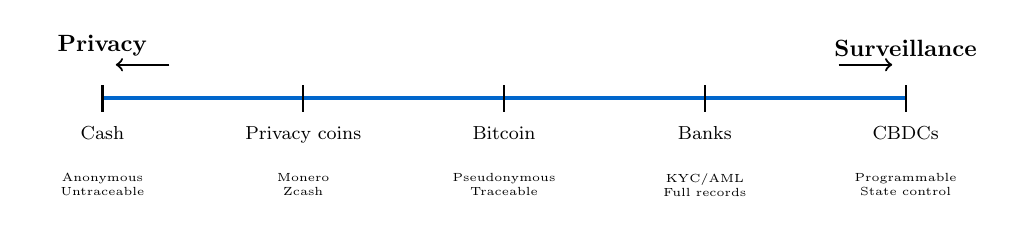
\begin{tikzpicture}[scale=0.85, transform shape]
% Spectrum line
\draw[ultra thick, dfblue] (0,0) -- (12,0);

% Markers
\foreach \x in {0,3,6,9,12} {
    \draw[thick] (\x,-0.2) -- (\x,0.2);
}

% Labels
\node[below] at (0,-0.3) {\footnotesize Cash};
\node[below] at (3,-0.3) {\footnotesize Privacy coins};
\node[below] at (6,-0.3) {\footnotesize Bitcoin};
\node[below] at (9,-0.3) {\footnotesize Banks};
\node[below] at (12,-0.3) {\footnotesize CBDCs};

% Arrow labels
\node[above] at (0,0.5) {\textbf{Privacy}};
\node[above] at (12,0.5) {\textbf{Surveillance}};
\draw[->, thick] (1,0.5) -- (0.2,0.5);
\draw[->, thick] (11,0.5) -- (11.8,0.5);

% Descriptions below
\node[below, text width=2cm, align=center, font=\tiny] at (0,-1) {Anonymous\\Untraceable};
\node[below, text width=2cm, align=center, font=\tiny] at (3,-1) {Monero\\Zcash};
\node[below, text width=2cm, align=center, font=\tiny] at (6,-1) {Pseudonymous\\Traceable};
\node[below, text width=2cm, align=center, font=\tiny] at (9,-1) {KYC/AML\\Full records};
\node[below, text width=2cm, align=center, font=\tiny] at (12,-1) {Programmable\\State control};
\end{tikzpicture}
\end{center}

\vspace{5mm}
\begin{block}{Key Question}
Where on this spectrum should financial systems be? Different societies, different answers.
\end{block}

\vspace{2mm}
\textbf{Note}: Most people assume they're somewhere in the middle---reality may differ.
\end{frame}

% ============================================================================
% SLIDE 6: Arguments for Financial Privacy
% ============================================================================
\begin{frame}{Arguments for Financial Privacy}
\begin{columns}[T]
\begin{column}{0.48\textwidth}
\textbf{Individual Rights:}
\begin{itemize}
\item Financial data reveals beliefs, health, relationships
\item Surveillance chills free expression
\item Protection from domestic abuse
\item Competitive business information
\item Freedom to make unpopular purchases
\end{itemize}

\vspace{3mm}
\textbf{Historical Precedent:}
\begin{itemize}
\item Nazi Germany: bank records used for persecution
\item Authoritarian states freeze activist accounts
\item Corporate surveillance for profit
\item Social credit systems emerge
\end{itemize}
\end{column}
\begin{column}{0.48\textwidth}
\textbf{Fungibility Principle:}
\begin{itemize}
\item Money should be interchangeable
\item ``Tainted'' coins create second-class money
\item Privacy preserves fungibility
\item Without fungibility, money becomes trackable assets
\end{itemize}

\vspace{3mm}
\begin{block}{Human Rights Perspective}
UN Declaration of Human Rights, Article 12:\\
``No one shall be subjected to arbitrary interference with his privacy.''
\end{block}
\end{column}
\end{columns}
\end{frame}

% ============================================================================
% SLIDE 7: Arguments for Financial Transparency
% ============================================================================
\begin{frame}{Arguments for Financial Transparency}
\begin{columns}[T]
\begin{column}{0.48\textwidth}
\textbf{Anti-Crime Rationale:}
\begin{itemize}
\item Money laundering enables crime
\item Terrorist financing prevention
\item Tax evasion detection
\item Sanctions enforcement
\item Fraud detection and recovery
\end{itemize}

\vspace{3mm}
\textbf{Consumer Protection:}
\begin{itemize}
\item Dispute resolution requires records
\item Fraud recovery needs traceability
\item Accountability for institutions
\item Insurance of deposits
\end{itemize}
\end{column}
\begin{column}{0.48\textwidth}
\textbf{Market Integrity:}
\begin{itemize}
\item Insider trading detection
\item Market manipulation prevention
\item Fair price discovery
\item Systemic risk monitoring
\end{itemize}

\vspace{3mm}
\begin{alertblock}{The AML Argument}
\$800B--\$2T laundered annually worldwide.\\
Transparency enables enforcement.\\
\vspace{2mm}
The controversial claim: ``Nothing to hide, nothing to fear.''
\end{alertblock}
\end{column}
\end{columns}
\end{frame}

% ============================================================================
% SLIDE 8: Privacy Technologies - Overview
% ============================================================================
\begin{frame}{Privacy Technologies in Cryptocurrency}
\begin{columns}[T]
\begin{column}{0.48\textwidth}
\textbf{Privacy Coins:}
\begin{itemize}
\item \textbf{Monero (XMR):} Ring signatures, stealth addresses, RingCT for amounts
\item \textbf{Zcash (ZEC):} zk-SNARKs, shielded transactions (optional)
\item \textbf{Dash:} CoinJoin mixing (PrivateSend)
\end{itemize}

\vspace{3mm}
\textbf{Mixing Services:}
\begin{itemize}
\item Tornado Cash (sanctioned by OFAC 2022)
\item CoinJoin implementations (Wasabi, JoinMarket)
\item Tumbling services (centralized, risky)
\end{itemize}
\end{column}
\begin{column}{0.48\textwidth}
\textbf{Zero-Knowledge Proofs:}
\begin{itemize}
\item Prove something without revealing it
\item ``I'm over 18'' without showing ID
\item ``I have funds'' without showing balance
\item ``I'm not sanctioned'' without revealing identity
\end{itemize}

\vspace{3mm}
\begin{block}{Emerging Possibility}
Privacy-preserving compliance: Prove you're compliant WITHOUT full surveillance. Technically possible, politically challenging.
\end{block}
\end{column}
\end{columns}
\end{frame}

% ============================================================================
% SLIDE 9: Zero-Knowledge Proofs Explained
% ============================================================================
\begin{frame}{Zero-Knowledge Proofs: Technical Foundation}
\begin{columns}[T]
\begin{column}{0.55\textwidth}
\textbf{What is a Zero-Knowledge Proof?}
\begin{itemize}
\item Cryptographic method where prover convinces verifier of a statement's truth
\item Without revealing ANY information beyond the truth itself
\item Neither party learns anything extra
\end{itemize}

\vspace{3mm}
\textbf{Classic Analogy: Color-Blind Friend}
\begin{enumerate}
\item Friend cannot distinguish red/green balls
\item You prove they're different colors
\item Without telling which is which
\item Repeated trials create confidence
\end{enumerate}
\end{column}
\begin{column}{0.42\textwidth}
\textbf{Financial Applications:}
\begin{itemize}
\item Prove age $\geq$ 18 without DOB
\item Prove balance $\geq$ X without showing balance
\item Prove not on sanctions list without revealing identity
\item Prove income meets threshold without disclosing amount
\end{itemize}

\vspace{3mm}
\begin{block}{Key Implementations}
\begin{itemize}
\item \textbf{zk-SNARKs}: Zcash, fast but trusted setup
\item \textbf{zk-STARKs}: No trusted setup, larger proofs
\item \textbf{Bulletproofs}: Monero's range proofs
\end{itemize}
\end{block}
\end{column}
\end{columns}
\end{frame}

% ============================================================================
% SLIDE 10: Monero Deep Dive
% ============================================================================
\begin{frame}{Privacy Coin Deep Dive: Monero (XMR)}
\begin{columns}[T]
\begin{column}{0.55\textwidth}
\textbf{Privacy Technologies Used:}
\begin{itemize}
\item \textbf{Ring Signatures:} Mix your transaction with decoys---sender hidden among group
\item \textbf{Stealth Addresses:} One-time addresses for each transaction---receiver unlinkable
\item \textbf{RingCT:} Confidential transactions hide amounts
\item \textbf{Dandelion++:} Network-level privacy for broadcast
\end{itemize}

\vspace{3mm}
\textbf{Result:}
\begin{itemize}
\item Sender, receiver, amount all hidden
\item Blockchain analysis extremely difficult
\item Default privacy (not optional like Zcash)
\end{itemize}
\end{column}
\begin{column}{0.42\textwidth}
\begin{alertblock}{Regulatory Response}
\begin{itemize}
\item Delisted from many exchanges
\item Japan, South Korea banned
\item Australia exchanges removed
\item IRS bounty for tracing (\$625K)
\end{itemize}
\end{alertblock}

\vspace{3mm}
\textbf{Use Cases:}
\begin{itemize}
\item Legitimate privacy needs
\item Dissidents and activists
\item Ransomware (unfortunately)
\item Tax evasion concerns
\end{itemize}
\end{column}
\end{columns}
\end{frame}

% ============================================================================
% SLIDE 11: Tornado Cash Case Study
% ============================================================================
\begin{frame}{Case Study: Tornado Cash Sanctions}
\begin{columns}[T]
\begin{column}{0.55\textwidth}
\textbf{What is Tornado Cash?}
\begin{itemize}
\item Ethereum mixing protocol (smart contract)
\item Users deposit ETH, withdraw to different address
\item Zero-knowledge proofs verify valid deposit
\item Breaks on-chain link between sender/receiver
\end{itemize}

\vspace{3mm}
\textbf{August 2022: OFAC Sanctions}
\begin{itemize}
\item US Treasury sanctions Tornado Cash
\item First time: sanctions on code/protocol, not entity
\item Developer arrested in Netherlands
\item GitHub repositories removed
\end{itemize}
\end{column}
\begin{column}{0.42\textwidth}
\textbf{The Debate:}
\begin{itemize}
\item \textbf{Government}: \$7B laundered, including North Korea hacks
\item \textbf{Critics}: Can you sanction open-source code? Neutral tool.
\end{itemize}

\vspace{3mm}
\begin{alertblock}{Legal Questions}
\begin{itemize}
\item Is code speech? (First Amendment)
\item Can immutable smart contracts be sanctioned?
\item What about users who need privacy legitimately?
\end{itemize}
\end{alertblock}

\vspace{2mm}
\textbf{2024 Update}: Court challenges ongoing.
\end{column}
\end{columns}
\end{frame}

% ============================================================================
% SLIDE 12: Blockchain Surveillance
% ============================================================================
\begin{frame}{Blockchain Surveillance: The Other Side}
\begin{columns}[T]
\begin{column}{0.55\textwidth}
\textbf{Blockchain Analysis Companies:}
\begin{itemize}
\item \textbf{Chainalysis}: Market leader, works with governments
\item \textbf{Elliptic}: UK-based, financial institutions
\item \textbf{TRM Labs}: Growing player
\item \textbf{CipherTrace}: Acquired by Mastercard
\end{itemize}

\vspace{3mm}
\textbf{Techniques Used:}
\begin{itemize}
\item \textbf{Clustering}: Link addresses to same entity
\item \textbf{Heuristics}: Common input ownership, change detection
\item \textbf{Exchange KYC}: Link to real identities
\item \textbf{IP tracking}: Network-level analysis
\end{itemize}
\end{column}
\begin{column}{0.42\textwidth}
\begin{block}{What They Can Do}
\begin{itemize}
\item Trace fund flows across chains
\item Identify exchange deposit addresses
\item Flag ``tainted'' coins
\item Link wallets to real identities
\item Build transaction graphs
\end{itemize}
\end{block}

\vspace{3mm}
\textbf{Key Insight:}\\
Bitcoin is \textbf{pseudonymous}, not anonymous. With enough data, most users can be identified.
\end{column}
\end{columns}
\end{frame}

% ============================================================================
% SLIDE 13: Pseudonymity vs Anonymity
% ============================================================================
\begin{frame}{Pseudonymity vs. Anonymity: Critical Distinction}
\begin{columns}[T]
\begin{column}{0.5\textwidth}
\textbf{Pseudonymity (Bitcoin, Ethereum):}
\begin{itemize}
\item Addresses are pseudonyms
\item All transactions publicly visible
\item Same address can be linked
\item Exchange KYC links to identity
\item Chain analysis can de-anonymize
\end{itemize}

\vspace{3mm}
\textbf{Common Misconception:}\\
Many users believe Bitcoin is ``anonymous.'' It is \textbf{not}---it's pseudonymous with a permanent, public transaction history.
\end{column}
\begin{column}{0.5\textwidth}
\textbf{Anonymity (Monero, Zcash shielded):}
\begin{itemize}
\item Sender hidden by ring signatures
\item Receiver hidden by stealth addresses
\item Amounts hidden by encryption
\item Linkage between transactions broken
\item Much harder (not impossible) to trace
\end{itemize}

\vspace{3mm}
\begin{alertblock}{Practical Reality}
Even ``anonymous'' systems have weaknesses:
\begin{itemize}
\item Exchange on/off ramps require KYC
\item IP addresses can be tracked
\item Human errors in OpSec
\end{itemize}
\end{alertblock}
\end{column}
\end{columns}
\end{frame}

% ============================================================================
% SLIDE 14: CBDCs - Surveillance Capabilities
% ============================================================================
\begin{frame}{CBDCs: The Ultimate Surveillance Tool?}
\begin{columns}[T]
\begin{column}{0.55\textwidth}
\textbf{CBDC Capabilities:}
\begin{itemize}
\item Complete transaction visibility
\item Programmable spending restrictions
\item Automatic tax collection
\item Expiring money (demurrage)
\item Geographic restrictions
\item Social credit integration
\item Remote freezing/confiscation
\end{itemize}

\vspace{3mm}
\textbf{China's e-CNY (Digital Yuan):}
\begin{itemize}
\item Real-time government visibility
\item Can be programmed for specific uses
\item Integrated with social systems
\item Pilot: 260M+ wallets active
\end{itemize}
\end{column}
\begin{column}{0.42\textwidth}
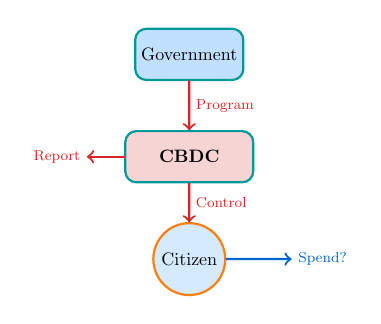
\begin{tikzpicture}[scale=0.65, transform shape]
% CBDC structure
\node (cbdc) [blockchain, minimum width=2.5cm, fill=dfred!20] {\textbf{CBDC}};
\node (gov) [blockchain, above of=cbdc, node distance=2cm, minimum width=2cm] {Government};
\node (citizen) [transaction, below of=cbdc, node distance=2cm] {Citizen};

\draw[->, thick, dfred] (cbdc) -- node[right, font=\footnotesize] {Control} (citizen);
\draw[->, thick, dfred] (gov) -- node[right, font=\footnotesize] {Program} (cbdc);
\draw[->, thick, dfblue] (citizen) -- ++(2,0) node[right, font=\footnotesize] {Spend?};
\draw[->, thick, dfred] (cbdc) -- ++(-2,0) node[left, font=\footnotesize] {Report};
\end{tikzpicture}

\vspace{3mm}
\begin{alertblock}{Dystopian Scenario}
Money that watches you, judges you, and can be remotely disabled or programmed.
\end{alertblock}
\end{column}
\end{columns}
\end{frame}

% ============================================================================
% SLIDE 15: CBDCs - Privacy Design Choices
% ============================================================================
\begin{frame}{CBDC Privacy: Design Choices Matter}
\begin{columns}[T]
\begin{column}{0.5\textwidth}
\textbf{Full Surveillance Model:}
\begin{itemize}
\item Central bank sees all transactions
\item Real-time monitoring possible
\item Maximum control and AML capability
\item Minimal user privacy
\item Example: China's e-CNY approach
\end{itemize}

\vspace{3mm}
\textbf{Tiered Privacy Model:}
\begin{itemize}
\item Small transactions anonymous
\item Larger transactions tracked
\item Balance limits without KYC
\item European approach (proposed)
\end{itemize}
\end{column}
\begin{column}{0.5\textwidth}
\textbf{Privacy-Preserving Model:}
\begin{itemize}
\item Zero-knowledge proofs for compliance
\item Central bank cannot see individual transactions
\item Only aggregate data visible
\item Technically challenging
\end{itemize}

\vspace{3mm}
\begin{block}{European Digital Euro Proposal}
\begin{itemize}
\item Offline capability for small payments
\item Privacy similar to cash for low-value
\item Higher thresholds require ID
\item Still under development (2024)
\end{itemize}
\end{block}
\end{column}
\end{columns}
\end{frame}

% ============================================================================
% SLIDE 16: Surveillance Capitalism
% ============================================================================
\begin{frame}{The Surveillance Capitalism Connection}
\begin{columns}[T]
\begin{column}{0.55\textwidth}
\textbf{Financial Data as Product:}
\begin{itemize}
\item Transaction data sold to advertisers
\item Credit scoring as control mechanism
\item Behavioral prediction markets
\item Insurance discrimination
\item Targeted pricing based on purchase history
\end{itemize}

\vspace{3mm}
\textbf{Corporate vs. State Surveillance:}
\begin{itemize}
\item PayPal, Visa see all transactions
\item Data shared with governments
\item No warrant needed for corporate data
\item ``Third-party doctrine'' (US)
\end{itemize}
\end{column}
\begin{column}{0.42\textwidth}
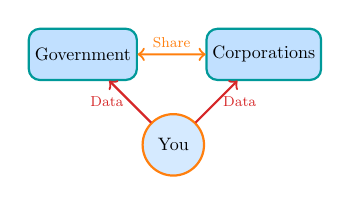
\begin{tikzpicture}[scale=0.65, transform shape]
% Surveillance triangle
\node (you) [transaction, minimum size=1.2cm] {You};
\node (corp) [blockchain, above right of=you, node distance=2.5cm, minimum width=2cm] {Corporations};
\node (gov) [blockchain, above left of=you, node distance=2.5cm, minimum width=2cm] {Government};

\draw[->, thick, dfred] (you) -- node[right, font=\footnotesize] {Data} (corp);
\draw[->, thick, dfred] (you) -- node[left, font=\footnotesize] {Data} (gov);
\draw[<->, thick, dforange] (corp) -- node[above, font=\footnotesize] {Share} (gov);
\end{tikzpicture}

\vspace{5mm}
\footnotesize
You are the product.\\
Your transactions are the data.\\
Privacy is the cost.
\end{column}
\end{columns}
\end{frame}

% ============================================================================
% SLIDE 17: Financial Inclusion - The Promise
% ============================================================================
\begin{frame}{The Financial Inclusion Promise}
\begin{columns}[T]
\begin{column}{0.55\textwidth}
\textbf{The Narrative:}
\begin{itemize}
\item 1.4 billion unbanked adults globally
\item Mobile phones reach areas banks don't
\item Crypto bypasses traditional gatekeepers
\item ``Bank the unbanked'' rallying cry
\item Permissionless access for all
\end{itemize}

\vspace{3mm}
\textbf{Success Stories:}
\begin{itemize}
\item M-Pesa in Kenya: 50M+ users
\item Remittances via stablecoins
\item Microloans via DeFi protocols
\item Cross-border payments simplified
\end{itemize}
\end{column}
\begin{column}{0.42\textwidth}
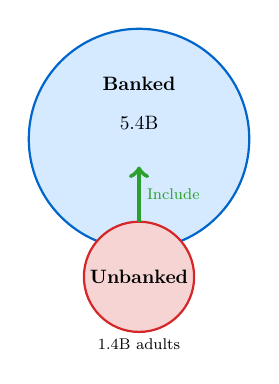
\begin{tikzpicture}[scale=0.7, transform shape]
% Inclusion diagram
\draw[thick, dfblue, fill=dflightblue4] (0,0) circle (2cm);
\node at (0,1) {\textbf{Banked}};
\node at (0,0.3) {5.4B};

\draw[thick, dfred, fill=dfred!20] (0,-2.5) circle (1cm);
\node at (0,-2.5) {\textbf{Unbanked}};
\node[below, font=\footnotesize] at (0,-3.5) {1.4B adults};

% Arrow
\draw[->, ultra thick, dfgreen] (0,-1.5) -- node[right, font=\footnotesize] {Include} (0,-0.5);
\end{tikzpicture}

\vspace{5mm}
\textbf{Key Question:}\\
Does digital finance actually serve the unbanked, or mainly the already-served?
\end{column}
\end{columns}
\end{frame}

% ============================================================================
% SLIDE 18: Financial Inclusion - Barriers
% ============================================================================
\begin{frame}{Financial Inclusion: Barriers That Remain}
\begin{columns}[T]
\begin{column}{0.48\textwidth}
\textbf{Traditional Barriers:}
\begin{itemize}
\item Geographic distance to banks
\item Documentation requirements (ID, proof of address)
\item Minimum balance requirements
\item High fees for small transactions
\item Lack of credit history
\item Language and literacy barriers
\end{itemize}
\end{column}
\begin{column}{0.48\textwidth}
\textbf{Digital Finance ``Solutions'' Create New Barriers:}
\begin{itemize}
\item Internet access required
\item Smartphone/device costs
\item Technical literacy needed
\item Complex UX excludes many
\item Gas fees price out small transactions
\item Volatility hurts the poor most
\item Regulatory uncertainty creates risk
\end{itemize}
\end{column}
\end{columns}

\vspace{3mm}
\begin{alertblock}{Critical Question}
Is crypto solving inclusion, or repackaging exclusion in new forms? The unbanked often become the ``un-crypto'd'' too.
\end{alertblock}
\end{frame}

% ============================================================================
% SLIDE 19: Financial Inclusion Critique
% ============================================================================
\begin{frame}{The Financial Inclusion Critique}
\begin{columns}[T]
\begin{column}{0.48\textwidth}
\textbf{Who Actually Benefits:}
\begin{itemize}
\item Tech-savvy early adopters
\item Those with capital to invest
\item Speculators and traders
\item People already financially included
\item Venture capital investors
\item Exchange operators
\end{itemize}

\vspace{3mm}
\textbf{New Exclusions Created:}
\begin{itemize}
\item Scams disproportionately hurt naive users
\item Rug pulls target newcomers
\item Complex DeFi requires expertise
\item No consumer protections
\end{itemize}
\end{column}
\begin{column}{0.48\textwidth}
\textbf{The ``Last Mile'' Problem:}
\begin{itemize}
\item On-ramps require KYC (excludes undocumented)
\item Off-ramps require bank accounts
\item Local currency conversion expensive
\item Merchant acceptance limited
\item User education lacking
\end{itemize}

\vspace{3mm}
\begin{block}{Reality Check}
Crypto adoption correlates more with speculation interest than financial exclusion. Turkey, Vietnam, Philippines: high adoption + existing financial access.
\end{block}
\end{column}
\end{columns}
\end{frame}

% ============================================================================
% SLIDE 20: Case Study - El Salvador
% ============================================================================
\begin{frame}{Case Study: El Salvador Bitcoin Experiment}
\begin{columns}[T]
\begin{column}{0.55\textwidth}
\textbf{What Happened (September 2021):}
\begin{itemize}
\item Bitcoin made legal tender
\item \$30 Bitcoin airdrop to citizens
\item Government-backed Chivo wallet
\item Volcano-powered mining announced
\end{itemize}

\vspace{3mm}
\textbf{Stated Goals:}
\begin{itemize}
\item Financial inclusion (70\% unbanked)
\item Cheaper remittances (20\% of GDP)
\item Attract investment and tourism
\item Reduce dollar dependence
\end{itemize}
\end{column}
\begin{column}{0.42\textwidth}
\textbf{Results (2024):}
\begin{itemize}
\item Daily use: limited adoption
\item Remittances: mostly traditional still
\item Volatility: government paper losses
\item IMF: ongoing concerns
\item Tourism: some ``crypto tourists''
\end{itemize}

\vspace{3mm}
\begin{block}{Verdict}
Mixed at best. Inclusion gains modest; volatility risks real; adoption limited to merchants near tourists. Not the revolution promised.
\end{block}
\end{column}
\end{columns}
\end{frame}

% ============================================================================
% SLIDE 21: M-Pesa Success Story
% ============================================================================
\begin{frame}{Success Story: M-Pesa (Not Crypto)}
\begin{columns}[T]
\begin{column}{0.55\textwidth}
\textbf{What is M-Pesa?}
\begin{itemize}
\item Mobile money platform (Kenya, 2007)
\item Works on basic feature phones via SMS
\item No smartphone or internet required
\item Agent network for cash-in/cash-out
\item Now: 50M+ users across Africa
\end{itemize}

\vspace{3mm}
\textbf{Why It Worked:}
\begin{itemize}
\item Built on existing infrastructure (SMS)
\item Local agent network (human touch)
\item Simple, intuitive interface
\item Regulatory support from Kenya
\item Addressed real needs (P2P transfers)
\end{itemize}
\end{column}
\begin{column}{0.42\textwidth}
\textbf{Inclusion Impact:}
\begin{itemize}
\item 2\% of Kenyans lifted from poverty
\item Women especially benefited
\item Rural access dramatically improved
\item Enabled small business growth
\end{itemize}

\vspace{3mm}
\begin{block}{The Lesson}
Financial inclusion success came from:
\begin{itemize}
\item Appropriate technology (not cutting-edge)
\item Human infrastructure (agents)
\item Regulatory cooperation
\item NOT from cryptocurrency
\end{itemize}
\end{block}
\end{column}
\end{columns}
\end{frame}

% ============================================================================
% SLIDE 22: Who Benefits, Who Is Harmed
% ============================================================================
\begin{frame}{Who Benefits? Who Is Harmed?}
\begin{center}
\renewcommand{\arraystretch}{1.3}
\begin{tabular}{|l|l|l|}
\hline
\textbf{Design Choice} & \textbf{Benefits} & \textbf{Harms} \\
\hline
Full transparency & Regulators, auditors & Privacy-seekers, dissidents \\
\hline
Full privacy & Individuals, activists & Law enforcement, crime victims \\
\hline
Pseudonymity (Bitcoin) & Moderate privacy seekers & Those needing true anonymity \\
\hline
CBDCs & Governments, AML & Individual autonomy \\
\hline
KYC requirements & Compliance, banks & Undocumented, unbanked \\
\hline
Permissionless access & Underserved, censored & May enable criminal use \\
\hline
\end{tabular}
\end{center}

\vspace{3mm}
\begin{alertblock}{No Neutral Design}
Every architectural choice has distributional consequences. Technology is not neutral---it embeds values and determines who wins and who loses.
\end{alertblock}
\end{frame}

% ============================================================================
% SLIDE 23: Privacy-Preserving Compliance
% ============================================================================
\begin{frame}{Emerging Privacy Solutions}
\begin{columns}[T]
\begin{column}{0.48\textwidth}
\textbf{Selective Disclosure:}
\begin{itemize}
\item Reveal only what's needed
\item Age verification without DOB
\item Solvency proof without balance
\item Compliance without surveillance
\end{itemize}

\vspace{3mm}
\textbf{Privacy-Preserving Compliance:}
\begin{itemize}
\item zk-proofs for sanctions screening
\item Encrypted transaction monitoring
\item Decentralized identity systems
\item Verifiable credentials
\end{itemize}
\end{column}
\begin{column}{0.48\textwidth}
\textbf{Example: Proving Non-Sanction}
\begin{enumerate}
\item Hash your identity locally
\item Prove hash NOT on OFAC list
\item Zero-knowledge proof sent to verifier
\item Never reveal actual identity
\end{enumerate}

\vspace{3mm}
\begin{block}{The Vision}
Compliance without surveillance. Privacy AND legitimacy. Technically possible, politically challenging, slowly emerging.
\end{block}
\end{column}
\end{columns}
\end{frame}

% ============================================================================
% SLIDE 24: Self-Sovereign Identity
% ============================================================================
\begin{frame}{Self-Sovereign Identity: A Middle Path?}
\begin{columns}[T]
\begin{column}{0.5\textwidth}
\textbf{What is Self-Sovereign Identity (SSI)?}
\begin{itemize}
\item Users control their own identity data
\item No reliance on centralized authority
\item Selective disclosure of attributes
\item Cryptographic verification
\end{itemize}

\vspace{3mm}
\textbf{How It Works:}
\begin{itemize}
\item Issuer provides verifiable credential
\item User stores in digital wallet
\item User presents proof to verifier
\item Verifier checks cryptographic validity
\end{itemize}
\end{column}
\begin{column}{0.5\textwidth}
\textbf{Financial Applications:}
\begin{itemize}
\item KYC once, use everywhere
\item Prove creditworthiness without revealing score
\item Age verification for services
\item Accredited investor status
\end{itemize}

\vspace{3mm}
\begin{block}{The Promise}
\begin{itemize}
\item User privacy enhanced
\item Compliance still achievable
\item Reduced data breach risk
\item Portable across services
\end{itemize}
\end{block}

\textbf{Projects}: Microsoft ION, Civic, Worldcoin (controversial)
\end{column}
\end{columns}
\end{frame}

% ============================================================================
% SLIDE 25: Day 5 Synthesis - Risk Framework
% ============================================================================
\begin{frame}{Day 5 Synthesis: The Risk Framework}
\begin{center}
\textbf{\Large For Any Digital Finance System, Ask:}
\end{center}

\vspace{5mm}
\begin{enumerate}
\item \textbf{Technical:} What can go wrong with the code/infrastructure?
\item \textbf{Economic:} What incentive attacks are possible?
\item \textbf{Human:} Who has power and might abuse it?
\item \textbf{Regulatory:} What jurisdiction risks exist?
\item \textbf{Governance:} Who decides changes, and how?
\item \textbf{Privacy:} Who sees what, and what can they do with it?
\item \textbf{Inclusion:} Who benefits, who is excluded, who is harmed?
\end{enumerate}

\vspace{5mm}
\begin{block}{The Critical Mindset}
Move from ``what can this do?'' to ``what can go wrong, and for whom?''
\end{block}
\end{frame}

% ============================================================================
% SLIDE 26: Day 5 Arc Summary
% ============================================================================
\begin{frame}{Day 5 Arc: From Failures to Values}
\begin{columns}[T]
\begin{column}{0.48\textwidth}
\textbf{What We Covered:}
\begin{enumerate}
\item \textbf{Failures (5.1):} Technical, economic, human failures in DeFi
\item \textbf{Regulation (5.2):} US fragmentation, EU MiCA, Asia divergence
\item \textbf{Governance (5.3):} DAO mechanisms and attack surfaces
\item \textbf{Privacy (5.4):} Surveillance vs. autonomy tradeoffs
\end{enumerate}
\end{column}
\begin{column}{0.48\textwidth}
\textbf{Key Takeaways:}
\begin{itemize}
\item Failures are inevitable---design for them
\item Regulation shapes what survives
\item Governance IS the attack surface
\item Privacy vs. transparency is political
\item Financial inclusion: promise vs. reality
\end{itemize}
\end{column}
\end{columns}

\vspace{5mm}
\begin{alertblock}{Day Arc}
What fails (5.1) $\rightarrow$ Who governs from outside (5.2) $\rightarrow$ Who governs from inside (5.3) $\rightarrow$ Who benefits and who is harmed (5.4)
\end{alertblock}
\end{frame}

% ============================================================================
% SLIDE 27: The Political Nature of Money
% ============================================================================
\begin{frame}{Additional Content: The Political Nature of Money}
\begin{columns}[T]
\begin{column}{0.5\textwidth}
\textbf{Money as Power:}
\begin{itemize}
\item Control over money = political power
\item Monetary policy shapes society
\item Financial access determines opportunity
\item Payment rails enable or restrict activity
\end{itemize}

\vspace{3mm}
\textbf{Historical Examples:}
\begin{itemize}
\item Bank derisking of legal industries
\item WikiLeaks payment processor ban
\item Convoy protests: frozen accounts
\item Nigerian #EndSARS donation blocks
\end{itemize}
\end{column}
\begin{column}{0.5\textwidth}
\textbf{Crypto as Political Statement:}
\begin{itemize}
\item Bitcoin: separation of money and state
\item Privacy coins: individual sovereignty
\item DeFi: financial system without gatekeepers
\item DAOs: new governance experiments
\end{itemize}

\vspace{3mm}
\begin{block}{The Core Question}
Who should control money?
\begin{itemize}
\item Governments (fiat, CBDCs)
\item Corporations (stablecoins, big tech)
\item Protocols (Bitcoin, Ethereum)
\item No one (cash, privacy coins)
\end{itemize}
\end{block}
\end{column}
\end{columns}
\end{frame}

% ============================================================================
% SLIDE 28: Global Privacy Perspectives
% ============================================================================
\begin{frame}{Additional Content: Global Privacy Perspectives}
\begin{columns}[T]
\begin{column}{0.5\textwidth}
\textbf{European Approach:}
\begin{itemize}
\item GDPR: Strong data protection
\item Digital Euro: Privacy by design (proposed)
\item Right to be forgotten
\item Data minimization principles
\end{itemize}

\vspace{3mm}
\textbf{US Approach:}
\begin{itemize}
\item Sectoral privacy laws
\item Third-party doctrine: less protection
\item Bank Secrecy Act: financial surveillance
\item No comprehensive federal privacy law
\end{itemize}
\end{column}
\begin{column}{0.5\textwidth}
\textbf{China Approach:}
\begin{itemize}
\item Digital Yuan: state visibility
\item Social credit integration
\item Tight capital controls
\item Crypto banned domestically
\end{itemize}

\vspace{3mm}
\begin{alertblock}{The Divergence}
Different societies reaching different conclusions:
\begin{itemize}
\item EU: Privacy as human right
\item US: Security/AML as priority
\item China: State control as goal
\item Crypto: Individual sovereignty
\end{itemize}
\end{alertblock}
\end{column}
\end{columns}
\end{frame}

% ============================================================================
% SLIDE 29: Discussion Questions
% ============================================================================
\begin{frame}{Discussion: Where Do You Stand?}
\begin{columns}[T]
\begin{column}{0.48\textwidth}
\textbf{Team Privacy Argues:}
\begin{itemize}
\item Privacy is a human right
\item Surveillance enables authoritarianism
\item Financial freedom requires anonymity
\item Technology should protect individuals
\item History shows surveillance abuse
\end{itemize}
\end{column}
\begin{column}{0.48\textwidth}
\textbf{Team Transparency Argues:}
\begin{itemize}
\item Privacy enables crime
\item Society needs accountability
\item Victims deserve recourse
\item ``Sunlight is the best disinfectant''
\item Democratic oversight requires visibility
\end{itemize}
\end{column}
\end{columns}

\vspace{5mm}
\begin{block}{Discussion Questions}
\begin{itemize}
\item Should there be a right to financial privacy? How absolute?
\item Who gets to decide the privacy-transparency tradeoff?
\item Is financial inclusion marketing or genuine social benefit?
\item Would you use a CBDC? Under what conditions?
\end{itemize}
\end{block}
\end{frame}

% ============================================================================
% SLIDE 30: Application - Personal Decisions
% ============================================================================
\begin{frame}{Application: Your Personal Privacy Choices}
\begin{columns}[T]
\begin{column}{0.5\textwidth}
\textbf{Questions to Consider:}
\begin{itemize}
\item What financial data do you generate daily?
\item Who has access to your transaction history?
\item What does your spending reveal about you?
\item How would you feel if it was public?
\end{itemize}

\vspace{3mm}
\textbf{Practical Steps:}
\begin{itemize}
\item Review privacy policies of financial apps
\item Consider data shared with third parties
\item Evaluate trade-offs of convenience vs. privacy
\item Understand your rights under local law
\end{itemize}
\end{column}
\begin{column}{0.5\textwidth}
\textbf{Framework for Evaluation:}
\begin{enumerate}
\item What data is collected?
\item Who has access?
\item How long is it retained?
\item Can it be deleted?
\item Is it sold to third parties?
\item What's the worst-case misuse?
\end{enumerate}

\vspace{3mm}
\begin{block}{Action Item}
Pick one financial service you use. Read its privacy policy. Understand what you're consenting to.
\end{block}
\end{column}
\end{columns}
\end{frame}

% ============================================================================
% SLIDE 31: Executive Summary
% ============================================================================
\begin{frame}{Executive Summary: Key Takeaways}
\begin{block}{The Five Things to Remember}
\begin{enumerate}
\item \textbf{Privacy-transparency is a spectrum}: Cash to CBDCs, with different tradeoffs at each point. No position is neutral.

\item \textbf{Technology embeds values}: Every design choice (privacy coins, CBDCs, KYC) has distributional consequences. Technology is political.

\item \textbf{Financial inclusion is complex}: 1.4B unbanked, but crypto adoption correlates more with speculation than solving exclusion. M-Pesa succeeded; El Salvador is mixed.

\item \textbf{Surveillance is multi-directional}: Governments AND corporations monitor transactions. You are the product.

\item \textbf{Privacy-preserving compliance is possible}: Zero-knowledge proofs offer a path to both privacy and regulatory compliance, but adoption is nascent.
\end{enumerate}
\end{block}

\vspace{2mm}
\textbf{Bottom Line}: The future of financial privacy is being decided now. Your values should inform your position.
\end{frame}

% ============================================================================
% SLIDE 32: Concept Map
% ============================================================================
\begin{frame}{Concept Map: Privacy, Surveillance, and Inclusion}
\begin{center}
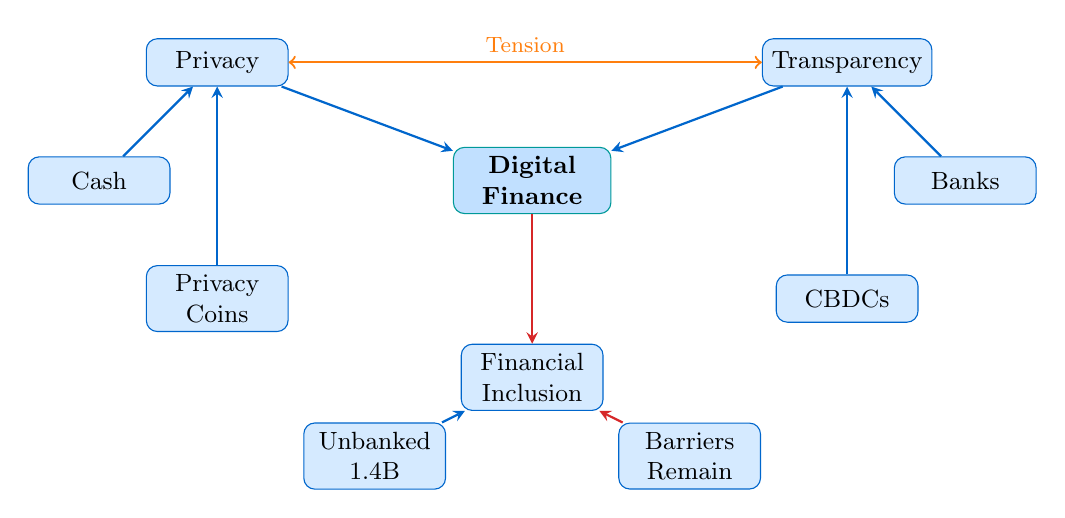
\begin{tikzpicture}[
    node distance=1.3cm,
    every node/.style={font=\small},
    box/.style={rectangle, rounded corners, draw=dfblue, fill=dflightblue4, minimum width=1.8cm, minimum height=0.6cm, align=center},
    bigbox/.style={rectangle, rounded corners, draw=dfteal, fill=dflightblue3, minimum width=2cm, minimum height=0.7cm, align=center, font=\small\bfseries}
]

% Central node
\node[bigbox] (center) at (0,0) {Digital\\Finance};

% Privacy side (left)
\node[box] (privacy) at (-4,1.5) {Privacy};
\node[box] (cash) at (-5.5,0) {Cash};
\node[box] (monero) at (-4,-1.5) {Privacy\\Coins};

% Transparency side (right)
\node[box] (transp) at (4,1.5) {Transparency};
\node[box] (banks) at (5.5,0) {Banks};
\node[box] (cbdc) at (4,-1.5) {CBDCs};

% Inclusion (bottom)
\node[box] (include) at (0,-2.5) {Financial\\Inclusion};
\node[box] (unbanked) at (-2,-3.5) {Unbanked\\1.4B};
\node[box] (barriers) at (2,-3.5) {Barriers\\Remain};

% Arrows
\draw[arrow] (privacy) -- (center);
\draw[arrow] (cash) -- (privacy);
\draw[arrow] (monero) -- (privacy);
\draw[arrow] (transp) -- (center);
\draw[arrow] (banks) -- (transp);
\draw[arrow] (cbdc) -- (transp);
\draw[arrow, dfred] (center) -- (include);
\draw[arrow] (unbanked) -- (include);
\draw[arrow, dfred] (barriers) -- (include);

% Tension arrow
\draw[<->, thick, dforange] (privacy) -- node[above] {\footnotesize Tension} (transp);

\end{tikzpicture}
\end{center}

\vspace{2mm}
\textcolor{dfred}{Red}: Challenges/gaps \quad \textcolor{dforange}{Orange}: Core tension
\end{frame}

% ============================================================================
% SLIDE 33: Key Terms (Part 1)
% ============================================================================
\begin{frame}{Key Terms \& Definitions (1/2)}
\begin{description}
\item[Financial Privacy] Control over who can see your financial transactions and data.

\item[Pseudonymity] Using identifiers (like Bitcoin addresses) not directly linked to real identity, but potentially traceable.

\item[Anonymity] True unlinkability between transactions and identity; much stronger than pseudonymity.

\item[Zero-Knowledge Proof] Cryptographic method to prove a statement is true without revealing any additional information.

\item[CBDC] Central Bank Digital Currency---digital money issued directly by a central bank, with various privacy models possible.
\end{description}
\end{frame}

% ============================================================================
% SLIDE 34: Key Terms (Part 2)
% ============================================================================
\begin{frame}{Key Terms \& Definitions (2/2)}
\begin{description}
\item[Privacy Coin] Cryptocurrency designed to hide transaction details (sender, receiver, amount). Examples: Monero, Zcash.

\item[Financial Inclusion] Providing access to useful, affordable financial services to underserved populations.

\item[KYC/AML] Know Your Customer / Anti-Money Laundering---regulatory requirements for identity verification.

\item[Self-Sovereign Identity] Identity model where individuals control their own data without centralized authority.

\item[Surveillance Capitalism] Economic system where personal data is collected and monetized, often without meaningful consent.
\end{description}

\vspace{3mm}
\textbf{Tip}: These terms are essential for discussing the ethical and political dimensions of digital finance.
\end{frame}

% ============================================================================
% SLIDE 35: Common Misconceptions
% ============================================================================
\begin{frame}{Common Misconceptions: Myth vs. Reality}
\begin{columns}[T]
\begin{column}{0.5\textwidth}
\begin{alertblock}{Myth 1}
``Bitcoin is anonymous.''
\end{alertblock}
\textbf{Reality}: Bitcoin is pseudonymous. All transactions are public. Chain analysis companies can often identify users.

\vspace{3mm}
\begin{alertblock}{Myth 2}
``Crypto will bank the unbanked.''
\end{alertblock}
\textbf{Reality}: Crypto adoption correlates more with speculation interest than financial exclusion. M-Pesa (not crypto) succeeded at inclusion.
\end{column}
\begin{column}{0.5\textwidth}
\begin{alertblock}{Myth 3}
``Privacy = criminal intent.''
\end{alertblock}
\textbf{Reality}: Privacy is a human right. Dissidents, abuse survivors, businesses, and ordinary people have legitimate privacy needs.

\vspace{3mm}
\begin{alertblock}{Myth 4}
``CBDCs are just digital cash.''
\end{alertblock}
\textbf{Reality}: CBDCs can have surveillance capabilities far beyond physical cash---programmable, trackable, freezable.
\end{column}
\end{columns}
\end{frame}

% ============================================================================
% SLIDE 36: Self-Assessment (1/2)
% ============================================================================
\begin{frame}{Self-Assessment: Test Your Understanding (1/2)}
\begin{block}{Question 1: Financial Barriers (Quiz Q3)}
What are common barriers to financial access for unbanked populations?
\begin{enumerate}[A)]
\item Lack of interest in financial services
\item Geographic distance to banks, high fees, documentation requirements, and lack of credit history
\item Government restrictions on all forms of money
\item Absence of currency in developing regions
\end{enumerate}
\end{block}

\vspace{2mm}
\pause
\textbf{Answer: B}---Barriers include physical distance, fees, ID requirements, and no credit history. These factors disproportionately affect low-income, rural, and marginalized populations.

\vspace{4mm}
\begin{block}{Question 2: Blockchain Surveillance (Quiz Q11)}
What tools enable blockchain surveillance and transaction tracking?
\begin{enumerate}[A)]
\item Only government intelligence agencies
\item Blockchain analysis tools like Chainalysis, Elliptic, and TRM Labs
\end{enumerate}
\end{block}
\pause
\textbf{Answer: B}---Commercial firms provide blockchain analysis to governments, exchanges, and financial institutions.
\end{frame}

% ============================================================================
% SLIDE 37: Self-Assessment (2/2)
% ============================================================================
\begin{frame}{Self-Assessment: Test Your Understanding (2/2)}
\begin{block}{Question 3: Cryptocurrency and Remittances (Quiz Q19)}
How can cryptocurrency potentially reduce remittance costs?
\begin{enumerate}[A)]
\item By eliminating all fees completely
\item Through peer-to-peer transfers using stablecoins, avoiding traditional correspondent banking networks and their fees
\item By increasing fees to improve service quality
\item Cryptocurrency cannot be used for remittances
\end{enumerate}
\end{block}

\vspace{2mm}
\pause
\textbf{Answer: B}---Traditional remittances cost 5--10\% through correspondent banking. Stablecoins enable direct P2P transfers with potentially lower fees, valuable for corridors where remittances are significant GDP share (e.g., 20\% for El Salvador).

\vspace{4mm}
\textbf{Reflection Questions:}
\begin{itemize}
\item Where on the privacy-transparency spectrum do you think finance should be?
\item What legitimate privacy needs exist beyond criminal use?
\item How should we balance inclusion promises against inclusion reality?
\end{itemize}
\end{frame}

% ============================================================================
% SLIDE 38: What's Next
% ============================================================================
\begin{frame}{What's Next: Day 6 -- Convergence and the Future}
\begin{columns}[T]
\begin{column}{0.5\textwidth}
\textbf{Preview: Where Is Digital Finance Going?}
\begin{itemize}
\item TradFi + DeFi convergence
\item Institutional adoption patterns
\item CBDCs and the future of money
\item AI + Finance integration
\item Your role in shaping this future
\end{itemize}

\vspace{3mm}
\textbf{Key Questions for Day 6:}
\begin{itemize}
\item What will survive regulatory scrutiny?
\item How will institutions and DeFi coexist?
\item What does 2030 finance look like?
\end{itemize}
\end{column}
\begin{column}{0.5\textwidth}
\begin{block}{Connection to This Topic}
\begin{itemize}
\item Privacy choices shape future adoption
\item Inclusion claims will be tested
\item CBDC designs will crystallize
\item Regulatory frameworks will mature
\end{itemize}
\end{block}

\vspace{2mm}
\textbf{Preparation:}
\begin{itemize}
\item Reflect: What would YOU build?
\item Think: What regulations would YOU write?
\item Consider: Whose values should prevail?
\end{itemize}
\end{column}
\end{columns}
\end{frame}

% ============================================================================
% SLIDE 39: Resources
% ============================================================================
\begin{frame}{Resources for Further Learning}
\begin{columns}[T]
\begin{column}{0.5\textwidth}
\textbf{Academic and Policy:}
\begin{itemize}
\item Chainalysis Crypto Crime Report (annual)
\item BIS papers on CBDCs and privacy
\item EU Digital Euro documentation
\item FATF Virtual Asset Guidance
\end{itemize}

\vspace{3mm}
\textbf{Books:}
\begin{itemize}
\item \textit{The Age of Surveillance Capitalism} (Zuboff)
\item \textit{Digital Cash} (Brunton)
\item \textit{The Bitcoin Standard} (Ammous)
\item \textit{Attack of the 50 Foot Blockchain} (Gerard)
\end{itemize}
\end{column}
\begin{column}{0.5\textwidth}
\textbf{Technical Deep Dives:}
\begin{itemize}
\item Monero whitepaper and documentation
\item Zcash protocol specification
\item Zero-knowledge proof tutorials (zkSNARKs)
\item Tornado Cash code (educational)
\end{itemize}

\vspace{3mm}
\textbf{News and Analysis:}
\begin{itemize}
\item CoinDesk, The Block (industry)
\item Molly White's Web3isgoinggreat.com (critical)
\item EFF on financial privacy
\item Privacy International
\end{itemize}

\vspace{3mm}
\textbf{Case Studies:}
\begin{itemize}
\item El Salvador Bitcoin adoption
\item M-Pesa in Kenya
\item China's Digital Yuan pilot
\end{itemize}
\end{column}
\end{columns}
\end{frame}

% ============================================================================
% SLIDE 40: Questions
% ============================================================================
\begin{frame}
\centering
\vspace{15mm}
{\Huge\textbf{Questions?}}

\vspace{10mm}
\textbf{Topic 5.4: Privacy, Surveillance, and Financial Inclusion}\\
\textit{Who Benefits and Who Is Harmed?}

\vspace{10mm}
\begin{block}{}
\centering
Joerg Osterrieder\\
Digital Finance\\
\texttt{joerg.osterrieder@ifi.uzh.ch}
\end{block}

\vspace{5mm}
\textbf{Next Up}: Day 6 -- Convergence and the Future
\end{frame}

\end{document}
